\chapter{עקומים ומשטחים ריבועיים}
בפרק זה נעסוק באפיון אלגברי של צורות גיאומטריות חשובות ונפוצות ב-$\bR^2$ ו-$\bR^3$. המשותף לכולן, הוא שניתן לבטאן כקבוצת האפסים של פולינומים ממעלות $2$ ו-$3$, בהתאמה.
\begin{definition}
יהיו $A,B$ קבוצות, ופונקציה $f:A\to B$. בהנתן $b\in B$, \textbf{קבוצת הרמה} של $f$ עבור הערך $b$ הוא הקבוצה
\[
	C_b=\qty{a\in A\middle|f(a)=b}.
\]
שימו לב כי הקבוצה $C_b$ עלולה להיות קבוצה ריקה.
\end{definition}
בקורס שלנו נעסוק בעיקר בקבוצות רמה של פונקציות מהצורה $f:\bR^2\to \bR$ או $f:\bR^3\to \bR$, ובמקרה זה נכנה את קבוצות הרמה המתאימות בשמות \textbf{קוי רמה} ו\textbf{משטחי רמה}.
\section{עקומים ריבועיים}
\begin{definition}
\textbf{פולינום ריבועי בשתי משתנים} הוא פונקציה מהצורה:
\[
	p(x,y)=ax^2+by^2+cxy+dx+ey+f
\]
\end{definition}
\begin{definition}
\textbf{עקום ריבועי} הוא קו-רמה של פולינום ריבועי. כלומר, קבוצה מהצורה:
\[
	C=\qty{\qty(x,y)\middle|ax^2+by^2+cxy+dx+ey+f=0},
\]
יחד עם ההנחה כי $a,b,c,d,e$ לא כולם אפס.
\end{definition}
לקבוצות אלו קוראים גם בשם \textbf{חתכים קוניים} שכן הם בדיוק העקומים שמתקבלים מהחיתוך של מישור וחרוט ב-$\bR^3$ (עד כדי סיבוב/שיקוף/הזזה). נעשה רדוקציה לצורה הכללית של עקום ריבועי על ידי שימוש בכך שכל משוואה ריבועית שקולה (עד כדי הפעלה של העתקה ליניארית והזזה) לאחת משלושת המשוואות הבאות:
\begin{enumerate}
\item $Ax^2+By^2+C=0$ כאשר $A,B$ לא שניהם אפס,
\item $Ax^2+By+C=0$ כאשר $A$ שונה מאפס,
\item $Ax+By+C=0$ כאשר $A,B$ לא שניהם אפס.
\end{enumerate}
עתה משביצענו רדוקציה לשלוש צורות פשוטות יחסית, נוכל לזהות את הצורה של הפתרונות.
\begin{enumerate}
\item \textbf{מעגל.} המשוואה \[x^2+y^2=R^2\] מתארת מעגל ברדיוס $R$ סביב ראשית הצירים. כאשר מחליפים את $(x,y)$ ב-$(x-x_0,y-y_0)$ במשוואה, מקבלים מעגל ברדיוס $R$ סביב הנקודה $(x_0,y_0)$.
\begin{figure}[h]
\begin{center}
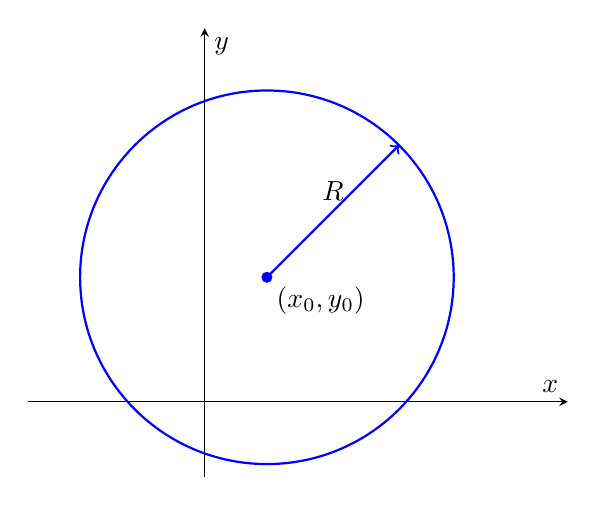
\begin{tikzpicture}
    % Define the center and the radius
    \def\xzero{1} % x_0
    \def\yzero{2} % y_0
    \def\radius{3} % R

    \begin{axis}[
        axis lines=middle,
        xmin=-2, xmax=5,
        ymin=-1.2, ymax=6,
        xlabel={$x$},
        ylabel={$y$},
        axis equal, % Ensures equal scaling for x and y axes
        ticks=none, % Removes the ticks from both axes
    ]

    % Draw the circle
    \draw[blue, thick] (\xzero,\yzero) circle (\radius);

    % Draw the center point
    \fill[blue] (\xzero,\yzero) circle (2pt) node[anchor=north west, black] {$(x_0,y_0)$};

    % Draw the radius with an arrow using curly braces for calculations
    \draw[->, thick, blue] (\xzero,\yzero) -- ({\xzero + \radius*cos(45)},{\yzero + \radius*sin(45)}) node[midway, above, black] {$R$};

    \end{axis}
\end{tikzpicture}
\label{ch1:fig1}
\caption{מעגל ברדיוס $R$ סביב הנקודה $(x_0,y_0)$.}
\end{center}
\end{figure}
\item \textbf{אליפסה.} אליפסה בעלת רוחב $2a$ ומוקדים $\qty(\pm c,0)$ מתארת את אוסף הנקודות שסכום מרחקן משני המוקדים קבוע ושווה ל-$2a$. המשוואה שמתארת את\linebreak האליפסה היא \[\frac{x^2}{a^2}+\frac{y^2}{b^2}=1\] כאשר $a^2-b^2=c^2$, ובמקרה זה הגובה של האליפסה הוא $2b$.
\begin{figure}[h]
\begin{center}
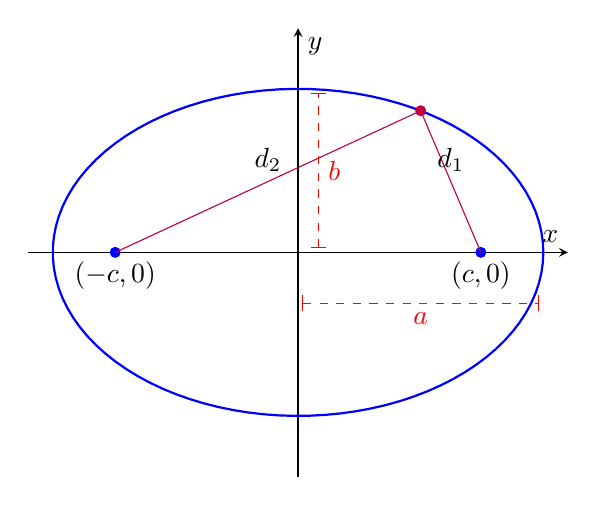
\begin{tikzpicture}
    % Define the ellipse parameters
    \def\a{3} % a
    \def\b{2} % b
    \pgfmathsetmacro{\c}{sqrt(\a^2 - \b^2)} % c

    \begin{axis}[
        axis lines=middle,
        xmin=-3.3, xmax=3.3,
        ymin=-2, ymax=2,
        xlabel={$x$},
        ylabel={$y$},
        axis equal, % Ensures equal scaling for x and y axes
        ticks=none, % Removes the ticks from both axes
    ]

    % Draw the ellipse
    \addplot[blue, thick, domain=0:360, samples=100] ({\a*cos(x)}, {\b*sin(x)});

    % Draw the points (c,0) and (-c,0)
    \fill[blue] (\c,0) circle (2pt) node[below, black] {$(c,0)$};
    \fill[blue] (-\c,0) circle (2pt) node[below, black] {$(-c,0)$};

    % Draw a point on the ellipse and lines connecting it to (c,0) and (-c,0)
    \coordinate (P) at ({\a*cos(60)}, {\b*sin(60)});
    \fill[purple] (P) circle (2pt);
    \draw[purple] (P) -- (\c,0) node[midway, above, black] {$d_1$};
    \draw[purple] (P) -- (-\c,0) node[midway, above, black] {$d_2$};

    % Draw lines indicating a and b
    \draw[red, dashed ,|-|] (0.05,-0.62) -- ({\a-0.05},-0.62) node[midway, below] {$a$};
    \draw[red, dashed ,|-|] (0.25,0.05) -- (0.25,{\b-0.05}) node[midway, right] {$b$};

    \end{axis}
\end{tikzpicture}
\label{ch1:fig2}
\caption{אליפסה עם רוחב $2a$ ואורך $2b$ כך שמתקיים $a^2-b^2=c^2$. לכל נקודה (בסגול) מתקיים $d_1+d_2=2a$.}
\end{center}
\end{figure}
\item \textbf{היפרבולה "עומדת".} היפרבולה בעלת מוקדים $\pm c$ ופרמטר $a>0$, מתארת את אוסף הנוקדות שהפרש המרחקים שלהן (בערך מוחלט) משני המוקדים קבוע, ושווה ל-$2a$. המשוואה שמתארת את ההיפרבולה היא \[\frac{x^2}{a^2}-\frac{y^2}{b^2}=1\] כאשר $a^2+b^2=c^2$.
\begin{enumerate}
	\item \textbf{היפרבולה "שוכבת".} זהה בהגדרתה להיפרבולה ה"עומדת" אך החלפנו את תפקידי הצירים. המשוואה המתארת את היפרבולה זו\linebreak היא \[\frac{y^2}{b^2}-\frac{x^2}{a^2}=1\].
	\item קיימת צורה נוספת להיפרבולה המסובבת בזווית $\frac{\pi}{4}$, ונתונה על ידי\linebreak המשוואה $xy=1$. שימו לב שניתן לזהות את משוואה זו כמשוואת היפרבולה בקלות אם נכתוב אותה באופן הבא:
	\[
		xy=\frac{(x+y)^2}{4}-\frac{\qty(x-y)^2}{4}=1.
	\]
	כלומר, זוהי היפרבולה שבה הצירים ה"טבעיים" הם הישרים $y=\pm x$.
\end{enumerate}
\begin{figure}[h]
    \centering
    % Top plot
    \begin{minipage}{\textwidth}
        \centering
        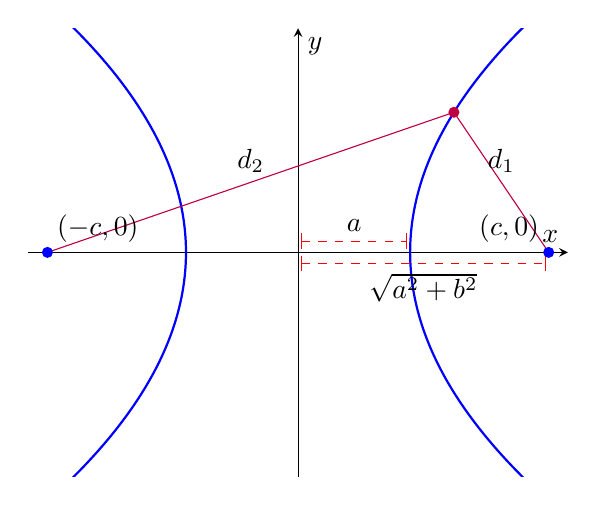
\begin{tikzpicture}
    % Define the hyperbola parameters
    \def\a{2} % a
    \def\b{4} % b
    \pgfmathsetmacro{\c}{sqrt(\a^2 + \b^2)} % c

    \begin{axis}[
        axis lines=middle,
        xmin=-4, xmax=4,
        ymin=-4, ymax=4,
        xlabel={$x$},
        ylabel={$y$},
        axis equal, % Ensures equal scaling for x and y axes
        ticks=none, % Removes the ticks from both axes
        samples=200
    ]

    % Draw the hyperbola
    \addplot[blue, thick, domain=0:{\c+1}] ({\a*(1+x^2/\b^2)},{x});
    \addplot[blue, thick, domain=0:{\c+1}] ({-\a*(1+x^2/\b^2)},{x});
    \addplot[blue, thick, domain=0:{\c+1}] ({\a*(1+x^2/\b^2)},{-x});
    \addplot[blue, thick, domain=0:{\c+1}] ({-\a*(1+x^2/\b^2)},{-x});

    % Draw the red dashed line from just above the origin to just above (a,0)
    \draw[red, dashed, |-|] (0.05,0.2) -- ({\a-0.05},0.2) node[midway, above, black] {$a$};

    % Draw the red dashed line from just below the origin to just below (c,0)
    \draw[red, dashed, |-|] (0.05,-0.2) -- ({\c-0.05},-0.2) node[midway, below, black] {$\sqrt{a^2+b^2}$};

    % Choose a point on the hyperbola and draw it in purple
    \coordinate (P) at ({\a*(1+2.5^2/\b^2)},2.5);
    \fill[purple] (P) circle (2pt);

    % Connect the point to (c,0) and (-c,0) and label the lines
    \draw[purple] (P) -- (\c,0) node[midway, above, black] {$d_1$};
    \draw[purple] (P) -- (-\c,0) node[midway, above, black] {$d_2$};

        % Draw the points (c,0) and (-c,0)
    \fill[blue] (\c,0) circle (2pt) node[above left, black] {$(c,0)$};
    \fill[blue] (-\c,0) circle (2pt) node[above right, black] {$(-c,0)$};

    \end{axis}
\end{tikzpicture}
    \end{minipage}
    
    \vspace{0.5cm} % Adjust this space as needed
    
    % Bottom left plot
    \begin{minipage}{0.48\textwidth}
        \centering
        \begin{tikzpicture}[scale=0.8]
    % Define the hyperbola parameters
    \def\a{4} % a
    \def\b{2} % b
    \pgfmathsetmacro{\c}{sqrt(\a^2 + \b^2)} % c

    \begin{axis}[
        axis lines=middle,
        xmin=-4, xmax=4,
        ymin=-4, ymax=4,
        xlabel={$x$},
        ylabel={$y$},
        axis equal, % Ensures equal scaling for x and y axes
        ticks=none, % Removes the ticks from both axes
        samples=200
    ]

    % Draw the hyperbola
    \addplot[blue, thick, domain=0:{\c+1}] ({x},{\b*(1+x^2/\a^2)});
    \addplot[blue, thick, domain=0:{\c+1}] ({x},{-\b*(1+x^2/\a^2)});
    \addplot[blue, thick, domain=0:{\c+1}] ({-x},{\b*(1+x^2/\a^2)});
    \addplot[blue, thick, domain=0:{\c+1}] ({-x},{-\b*(1+x^2/\a^2)});

    \end{axis}
\end{tikzpicture}
    \end{minipage}
    \hfill
    % Bottom right plot
    \begin{minipage}{0.48\textwidth}
        \centering
        \begin{tikzpicture}[scale=0.8]
    % Define the hyperbola parameters
    \def\a{4} % a
    \def\b{2} % b
    \pgfmathsetmacro{\c}{sqrt(\a^2 + \b^2)} % c

    \begin{axis}[
        axis lines=middle,
        xmin=-4, xmax=4,
        ymin=-4, ymax=4,
        xlabel={$x$},
        ylabel={$y$},
        axis equal, % Ensures equal scaling for x and y axes
        ticks=none, % Removes the ticks from both axes
        samples=200
    ]

    % Draw the hyperbola
    \addplot[blue, thick, domain={1/3.5}:3.5] ({x},{1/x});
	\addplot[blue, thick, domain={1/3.5}:3.5] ({-x},{-1/x});
    \end{axis}
\end{tikzpicture}
    \end{minipage}
    \label{ch1:fig3}    
    \caption{היפרבולה "עומדת" (בגרף העליון) עם פרמטר $a$ ופרמטר $b$ שעבורו $a^2+b^2=c^2$. כל נקודה על ההיפרבולה (בסגול) מקיימת $\qty|d_1-d_2|=2a$. משמאל למטה ניתן לראות היפרבולה שוכבת ומימין למטה $xy=1$.}

\end{figure}
\item \textbf{פרבולה.} עבור פרמטר $p\neq 0$, הפרבולה היא אוסף הנקודות שמרחקן מהמוקד $\qty(\frac{p}{2},0)$ שווה למרחקן מהישר $x=-\frac{p}{2}$. משוואת הפרבולה היא \[y^2=2px\].
\begin{figure}[h]
\begin{center}
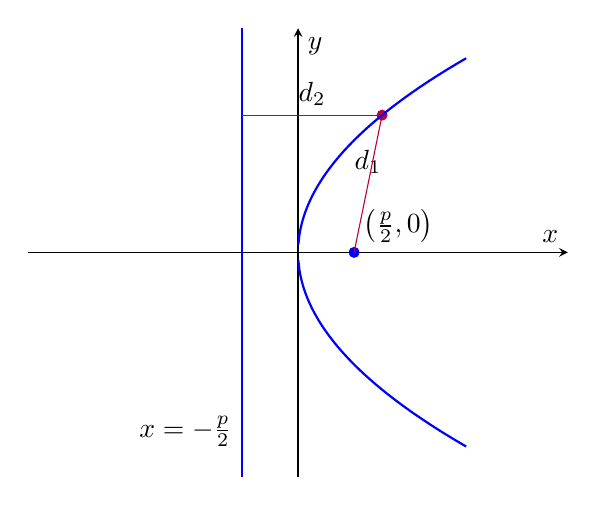
\begin{tikzpicture}
    % Define the parabola parameter
    \def\p{2}

    \begin{axis}[
        axis lines=middle,
        xmin=-3, xmax=3,
        ymin=-4, ymax=4,
        xlabel={$x$},
        ylabel={$y$},
        axis equal, % Ensures equal scaling for x and y axes
        ticks=none, % Removes the ticks from both axes
        samples=200,
        domain=-1:3 % Adjust the domain as needed
    ]
    % Draw the point (p/2,0)
    \fill[blue] (\p/2,0) circle (2pt) node[above right, black] {$\left(\frac{p}{2},0\right)$};

    % Draw the line x=-p/2
    \addplot[blue, thick, domain=-4:4] (-\p/2, x) node[pos=0.1, left, black] {$x=-\frac{p}{2}$};

    % Choose a point on the parabola
    \coordinate (P) at (1.5,{sqrt(2*\p*1.5)});
    \fill[purple] (P) circle (2pt);
    
    % Connect the point to (p/2,0) and to the line x=-p/2
    \draw[purple] (P) -- (\p/2,0) node[midway, above, black] {$d_1$};
    \draw[purple] (P) -- (-\p/2,{sqrt(2*\p*1.5)}) node[midway, above, black] {$d_2$};

    % Draw the parabola
    \addplot[blue, thick] ({x},{sqrt(2*\p*x)});
    \addplot[blue, thick] ({x},{-sqrt(2*\p*x)});

    \end{axis}
\end{tikzpicture}
\label{ch1:fig4}
\caption{פרבולה עם פרמטר $p$. כל נקודה על הפרבולה (בסגול) מקיימת $d_1=d_2$.}
\end{center}
\end{figure}
\item \textbf{קו ישר יחיד.} בהנתן כיוון $\qty(a,b)$ ופרמטר $d\geq 0$, הישר $ax+by+d=0$ הוא הישר שניצב לכיוון $\qty(a,b)$ ומרחקו $d$ מראשית הצירים.
\item \textbf{זוג קווים ישרים.} ניתן לקבל זוג קווים ישרים באחד מהמקרים הבאים:
\begin{enumerate}
\item $(ax+by+d)^2=c^2$ וגם $c>0$. במקרה זה מתקבלים שני הישרים המקבילים $ax+by+d=\pm c$.
\item $(ax+by+d)(\alpha x+\beta y+\gamma)=0$. במקרה זה מתקבלים שני ישרים נחתכים.
\end{enumerate}
\item \textbf{נקודה בודדת.} מתקבלת כאשר המשוואה מהצורה $ax^2+by^2=0$ וגם $a,b$ בעלי אותו סימן.
\item \textbf{קבוצה ריקה.} מתקבלת כאשר המשוואה מהצורה $ax^2+by^2=-c^2$ כאשר $a,b$ אי שליליים ולא שניהם אפס, וכאשר $c$ אינו אפס.
\end{enumerate}
נזכיר כי כל הצורות שתיארנו כאן מובאות בגרסתן הפשוטה ביותר. באופן כללי, כל אחת מהצורות עלולה להופיע בצורה מסובבת, מוזזת או משוקפת. כך למשל, המשוואה:
\[
	\frac{\qty(\cos{(\theta)}x-\sin{(\theta)}y)^2}{4}+\frac{\qty(\sin{(\theta)}x+\cos{(\theta)}y)^2}{9}=1
\]
מתארת אליפסה בעלת רוחב $2$ ואורך $3$, מסובבת ב-$\theta$ עם כיוון השעון.
\section{משטחים ריבועיים}
\begin{definition}
\textbf{פולינום ריבועי בשלושה משתנים} הוא פונקציה מהצורה:
\[
	p(x,y,z)=Ax^2+By^2+Cz^2+Dxy+Eyz+Fzx+Gx+Hy+Iz+J.
\]
\end{definition}
\begin{definition}
\textbf{משטח ריבועי} הוא משטח-רמה של פולינום ריבועי בשלושה משתנים. כלומר, קבוצה מהצורה:
\[
	C=\qty{\qty(x,y,z)\middle|p(x,y,z)=0}.
\]
כאשר $p(x,y,z)$ פולינום ריבועי ולא קבוע.
\end{definition}
בדומה לעקומים ריבועיים, גם את המשטחים הריבועיים ניתן להביא למספר צורות קנוניות, וגם המשטחים הריבועיים מהווים \textbf{חתך קוני}, כך שהם כולם מתקבלים על ידי חיתוך של על-מישור ב-$\bR^4$ עם חרוט. לבסוף, עד כדי רדוקציה דומה לזו שעשינו עבור עקומים ריבועיים, נוכל לתאר את הצורות האפשריות של משטחים ריבועיים.
\begin{enumerate}
\item \textbf{ספירה.} המשוואה
\[
	x^2+y^2+z^2=R^2
\]
והיא מתארת קליפה של כדור תלת ממדי ברדיוס $R$ סביב הראשית. גם כאן, ניתן להחליף את $(x,y,z)$ ב-$(x-x_0,y-y_0,z-z_0)$ ולקבל כדור מוזז שמרכזו בנקודה $(x_0,y_0,z_0)$.
\item \textbf{אליפסואיד.} המשוואה
\[
	\frac{x^2}{a^2}+\frac{y^2}{b^2}+\frac{z^2}{c^2}=1
\]
מתארת אליפסואיד בעל רוחב $2a,2b,2c$ בשלושת הצירים בהתאמה.
\item \textbf{משטחים בעלי חתכי גובה אליפטיים.} הם משטחים שהחיתוך שלהם עם המישורים $z=C$ הינם אליפסות.
\begin{enumerate}
\item \textbf{חרוט אליפטי.} פתרונות המשוואה
\[
	\frac{x^2}{a^2}+\frac{y^2}{b^2}-\frac{z^2}{c^2}=0
\]
מקיימים שלכל ערך קבוע של $z$, מתקבלת משוואת אליפסה, וככל ש-$\qty|z|$ גדל, כך האליפסה גדלה (ומכאן השם חרוט אליפטי, כלומר, חרוט שחתכי הגובה שלו הן אליפסות).
\item \textbf{גליל אליפטי.} בדומה לחרוט האליפטי, גם משטח זה מקיים שחתכי הגובה שלו הן אליפסות. אך הוא נתון על ידי המשוואה:
\[
	\frac{x^2}{a^2}+\frac{y^2}{b^2}=1
\]
כלומר, $z$ אינו משחק תפקיד ויכול לקבל כל ערך שהוא רוצה. יתרה מכך, גודל האליפסות בחתכי הגובה אינו משתנה/תלוי ב-$z$, ולכן מתקבלת הצורה הגלילית שבאיור לעיל.
\item \textbf{פרבולואיד אליפטי.} בהמשך לצורות שחתכי הגובה שלהן אליפסות, גם כאן מדובר בצורה דומה, אלא שגודל האליפסות משתנה לפי שורש הגודל של $z$. המשוואה המתארת פרבולואיד אליפטי היא:
\[
	\frac{x^2}{a^2}+\frac{y^2}{b^2}-z=0.
\]
\end{enumerate}
\item \textbf{משטחים בעלי חתכי גובה היפרבוליים.} דומים מאוד בצורתם לאלו האליפטיים, כאשר אחד מהמקדמים בפולינום בסימן הפוך.
\begin{enumerate}
\item \textbf{גליל היפרבולי.} נתון על ידי המשוואה $\frac{x^2}{a^2}-\frac{y^2}{b^2}=-1$, כך שבדומה לגליל האליפטי $z$ אינו משחק תפקיד כלל.
\item \textbf{פרבולואיד היפרבולי.} נתון על ידי המשוואה $z=\frac{y^2}{b^2}-\frac{x^2}{a^2}$.
\end{enumerate}
\item \textbf{היפרבולואיד חד-יריעתי ודו-יריעתי.} ההיפרבולואיד החד-יריעתי נתון על ידי המשוואה:
\[
	\frac{x^2}{a^2}+\frac{y^2}{b^2}-\frac{z^2}{c^2}=1.
\]
וההיפרבולואיד הדו יריעתי נתון על ידי המשוואה:
\[
	\frac{x^2}{a^2}+\frac{y^2}{b^2}-\frac{z^2}{c^2}=-1.
\]
ההבדל ביניהם, כמתואר באיורים שלעיל, הוא בכך שההיפרבולואיד החד יריעתי מהווה משטח אחד "מחובר" (בהמשך, נקרא לזה בשם "קשיר"), וההיפרבולואיד הדו יריעתי מורכב משני משטחים נפרדים וזרים (בפרט, נאמר שהוא "אינו קשיר").
\item \textbf{גליל פרבולי.} נתון על ידי משוואה מהצורה $x^2+2rz=0$ עם פרמטר $r\neq 0$.
\item \textbf{מישורים.} המשוואה $\qty(ax+by+cz+d)^2=r^2$ מתארת מישור יחיד אם $r=0$, ושני מישורים מקבילים אם $r\neq 0$. קיימת גם אפשרות של מישורים נחתכים, כאשר הצורה הכללית ביותר למשוואה כזו היא
\[
	\qty(ax+by+cz+d)\qty(\alpha x+\beta y+\gamma z+\delta)=0.
\]
\end{enumerate}

% Sphere and Ellipsoid
\begin{figure}[h]
	\definecolor{lightblue}{rgb}{0.53, 0.81, 0.98}
    \centering
    % First plot
    \begin{minipage}{0.45\textwidth}
        \centering
        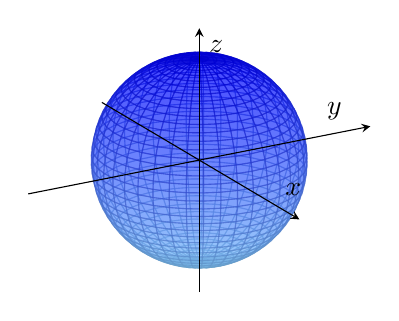
\begin{tikzpicture}
    \begin{axis}[
        view={60}{20}, % Adjust the viewing angle
        axis lines=center,
        axis on top,
        axis equal,
        xlabel={$x$},
        ylabel={$y$},
        zlabel={$z$},
        xmin=-1.25, xmax=1.3,
        ymin=-1, ymax=1,
        zmin=-1.3, zmax=1.3,
        ticks=none, % Removes the ticks from all axes
        colormap={blues}{color(0cm)=(lightblue); color(1cm)=(blue)} % Define a blue gradient colormap
    ]
    \addplot3[
        surf,
        opacity=0.5, % Adjust the transparency
        samples=40, % Adjust the number of samples for better resolution
        domain=0:pi, y domain=0:2*pi,
        z buffer=sort
    ] ({sin(deg(x))*cos(deg(y))}, {sin(deg(x))*sin(deg(y))}, {cos(deg(x))});
    \end{axis}
\end{tikzpicture}
\label{ch1:fig5}
\caption{ספירה.}
    \end{minipage}
    \hfill % Optional: to ensure horizontal spacing between the plots
    % Second plot
    \begin{minipage}{0.45\textwidth}
        \centering
        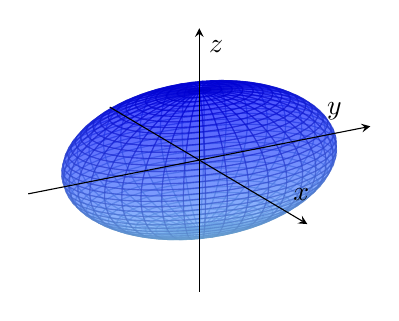
\begin{tikzpicture}
    \begin{axis}[
        view={60}{20}, % Adjust the viewing angle
        axis lines=center,
        axis on top,
        axis equal,
        xlabel={$x$},
        ylabel={$y$},
        zlabel={$z$},
        xmin=-2.25, xmax=3,
        ymin=-4, ymax=4,
        zmin=-1.75, zmax=1.75,
        ticks=none, % Removes the ticks from all axes
        colormap={blues}{color(0cm)=(lightblue); color(1cm)=(blue)} % Define a blue gradient colormap
    ]
    \addplot3[
        surf,
        opacity=0.5, % Adjust the transparency
        samples=40, % Adjust the number of samples for better resolution
        domain=0:pi, y domain=0:2*pi,
        z buffer=sort
    ] ({2*sin(deg(x))*cos(deg(y))}, {3*sin(deg(x))*sin(deg(y))}, {1.5*cos(deg(x))});
    \end{axis}
\end{tikzpicture}
\label{ch1:fig6}
\caption{אליפסואיד.}
    \end{minipage}
\end{figure}

% Elliptic Cone and Cylinder
\begin{figure}
	\definecolor{lightblue}{rgb}{0.53, 0.81, 0.98}
    \centering
    % First plot
    \begin{minipage}{0.45\textwidth}
        \centering
        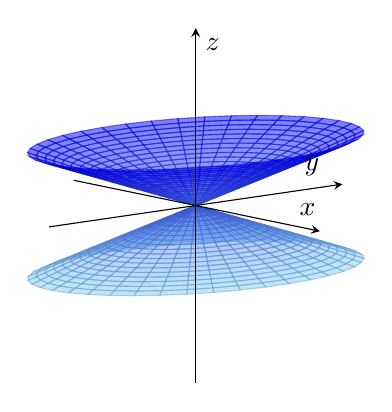
\begin{tikzpicture}
    \begin{axis}[
        view={50}{10}, % Adjust the viewing angle
        axis lines=center,
        axis on top,
        axis equal,
        xlabel={$x$},
        ylabel={$y$},
        zlabel={$z$},
        xmin=-2.25, xmax=2.3,
        ymin=-3, ymax=3,
        zmin=-1.3, zmax=1.3,
        ticks=none, % Removes the ticks from all axes
        colormap={blues}{color(0cm)=(lightblue); color(1cm)=(blue)} % Define a blue gradient colormap
    ]
    \addplot3[
        surf,
        opacity=0.5, % Adjust the transparency
        samples=40, % Adjust the number of samples for better resolution
        domain=-1:1, y domain=0:2*pi,
        z buffer=sort
    ] ({2*x*cos(deg(y))}, {3*x*sin(deg(y))}, {x});
    \end{axis}
\end{tikzpicture}
\label{ch1:fig7}
\caption{חרוט אליפטי.}
    \end{minipage}
    \hfill % Optional: to ensure horizontal spacing between the plots
    % Second plot
    \begin{minipage}{0.45\textwidth}
        \centering
        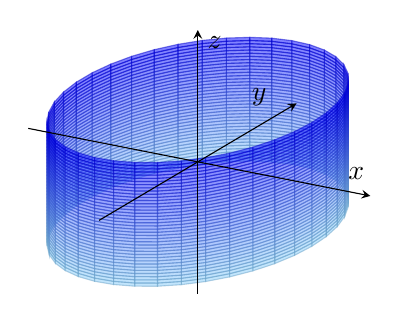
\begin{tikzpicture}
    \begin{axis}[
        view={30}{20}, % Adjust the viewing angle
        axis lines=center,
        axis on top,
        axis equal,
        xlabel={$x$},
        ylabel={$y$},
        zlabel={$z$},
        xmin=-2.25, xmax=2.3,
        ymin=-3, ymax=3,
        zmin=-1.3, zmax=1.3,
        ticks=none, % Removes the ticks from all axes
        colormap={blues}{color(0cm)=(lightblue); color(1cm)=(blue)} % Define a blue gradient colormap
    ]
    \addplot3[
        surf,
        opacity=0.5, % Adjust the transparency
        samples=40, % Adjust the number of samples for better resolution
        domain=-1:1, y domain=0:2*pi,
        z buffer=sort
    ] ({2*cos(deg(y))}, {3*sin(deg(y))}, {x});
    \end{axis}
\end{tikzpicture}
\label{ch1:fig8}
\caption{גליל אליפטי.}
    \end{minipage}
\end{figure}

% Elliptic Parabolloid and Hyperbollic Parabolloid
\begin{figure}
	\definecolor{lightblue}{rgb}{0.53, 0.81, 0.98}
    \centering
    % First plot
    \begin{minipage}{0.45\textwidth}
        \centering
        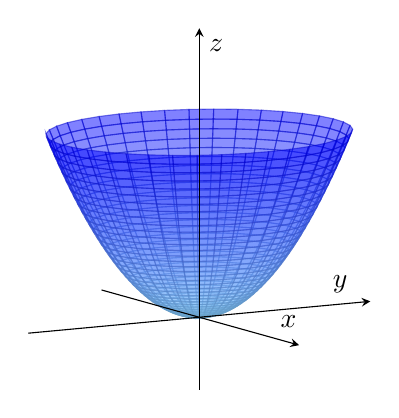
\begin{tikzpicture}
    \begin{axis}[
        view={60}{10}, % Adjust the viewing angle
        axis lines=center,
        axis on top,
        xlabel={$x$},
        ylabel={$y$},
        zlabel={$z$},
        xmin=-2.25, xmax=2.3,
        ymin=-3, ymax=3,
        zmin=-0.25, zmax=1,
        ticks=none, % Removes the ticks from all axes
        colormap={blues}{color(0cm)=(lightblue); color(1cm)=(blue)} % Define a blue gradient colormap
    ]
    \addplot3[
        surf,
        opacity=0.5, % Adjust the transparency
        samples=40, % Adjust the number of samples for better resolution
        domain=0:0.8, y domain=0:2*pi,
        z buffer=sort
    ] ({2*x*cos(deg(y))}, {3*x*sin(deg(y))}, {x^2});
    \end{axis}
\end{tikzpicture}
\label{ch1:fig9}
\caption{פרבולואיד אליפטי.}
    \end{minipage}
    \hfill % Optional: to ensure horizontal spacing between the plots
    % Second plot
    \begin{minipage}{0.45\textwidth}
        \centering
        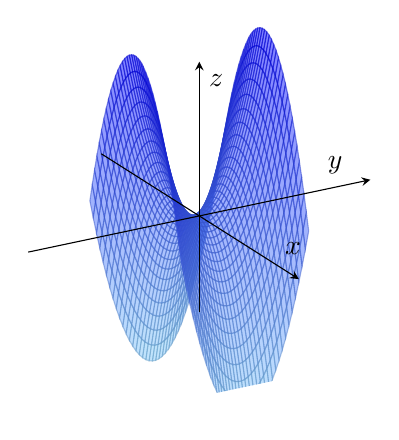
\begin{tikzpicture}
    \begin{axis}[
        view={60}{30}, % Adjust the viewing angle
        axis lines=center,
        axis on top,
        xlabel={$x$},
        ylabel={$y$},
        zlabel={$z$},
        xmin=-3.25, xmax=3.3,
        ymin=-4, ymax=4,
        zmin=-1.25, zmax=2,
        ticks=none, % Removes the ticks from all axes
        colormap={blues}{color(0cm)=(lightblue); color(1cm)=(blue)} % Define a blue gradient colormap
    ]
    \addplot3[
        surf,
        opacity=0.5, % Adjust the transparency
        samples=40, % Adjust the number of samples for better resolution
        domain=-1.5:1.5, y domain=-1.5:1.5,
        z buffer=sort
    ] ({x},{y},{y^2-x^2});
    \end{axis}
\end{tikzpicture}
		\label{ch1:fig11}
		\caption{פרבולואיד היפרבולי.}
    \end{minipage}
\end{figure}

% Hyperbollic and Parabollic Cylinder
\begin{figure}
	\definecolor{lightblue}{rgb}{0.53, 0.81, 0.98}
    \centering
    % First plot
    \begin{minipage}{0.45\textwidth}
        \centering
        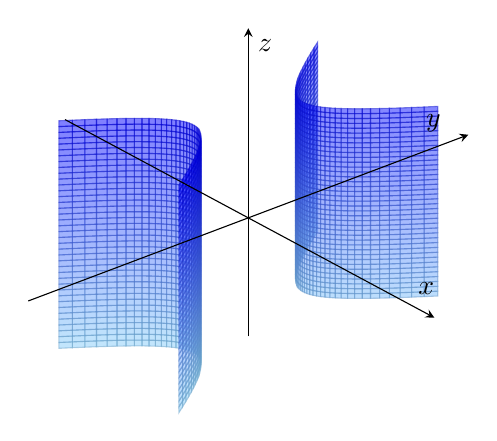
\begin{tikzpicture}
    \begin{axis}[scale=1.5,
        view={50}{40}, % Adjust the viewing angle
        axis lines=center,
        axis on top,
        xlabel={$x$},
        ylabel={$y$},
        zlabel={$z$},
        xmin=-3.25, xmax=3.3,
        ymin=-4, ymax=4,
        zmin=-1.25, zmax=2,
        ticks=none, % Removes the ticks from all axes
        colormap={blues}{color(0cm)=(lightblue); color(1cm)=(blue)} % Define a blue gradient colormap
    ]
    \addplot3[
        surf,
        opacity=0.5, % Adjust the transparency
        samples=40, % Adjust the number of samples for better resolution
        domain=-1.5:1.5, y domain=-1:1,
        z buffer=sort
    ] ({0.5*sinh(x)},{cosh(x)},{y});
    \addplot3[
        surf,
        opacity=0.5, % Adjust the transparency
        samples=40, % Adjust the number of samples for better resolution
        domain=-1.5:1.5, y domain=-1.2:1.2,
        z buffer=sort
    ] ({0.5*sinh(x)},{-cosh(x)},{y});
    \end{axis}
\end{tikzpicture}
\label{ch1:fig12}
\caption{גליל היפרבולי.}
    \end{minipage}
    \hfill % Optional: to ensure horizontal spacing between the plots
    % Second plot
    \begin{minipage}{0.45\textwidth}
        \centering
        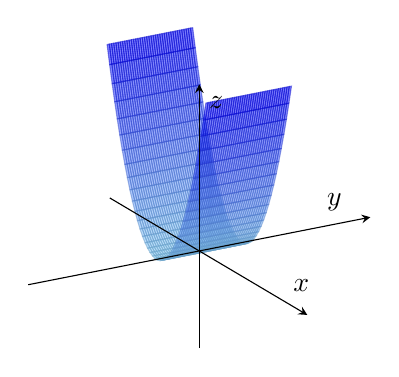
\begin{tikzpicture}
    \begin{axis}[
        view={60}{20}, % Adjust the viewing angle
        axis lines=center,
        axis on top,
        axis equal,
        xlabel={$x$},
        ylabel={$y$},
        zlabel={$z$},
        xmin=-2.25, xmax=3,
        ymin=-4, ymax=4,
        zmin=-0.25, zmax=1.75,
        ticks=none, % Removes the ticks from all axes
        colormap={blues}{color(0cm)=(lightblue); color(1cm)=(blue)} % Define a blue gradient colormap
    ]
    \addplot3[
        surf,
        opacity=0.5, % Adjust the transparency
        samples=40, % Adjust the number of samples for better resolution
        domain=-2:2, y domain=-1:1,
        z buffer=sort
    ] ({x}, {y}, {x^2});
    \end{axis}
\end{tikzpicture}
\label{ch1:fig15}
\caption{גליל פרבולי.}
    \end{minipage}
\end{figure}

% Hyperbolloid
\begin{figure}[h]
    \centering
    % First plot
    \begin{minipage}{0.45\textwidth}
        \centering
        \definecolor{lightblue}{rgb}{0.53, 0.81, 0.98}
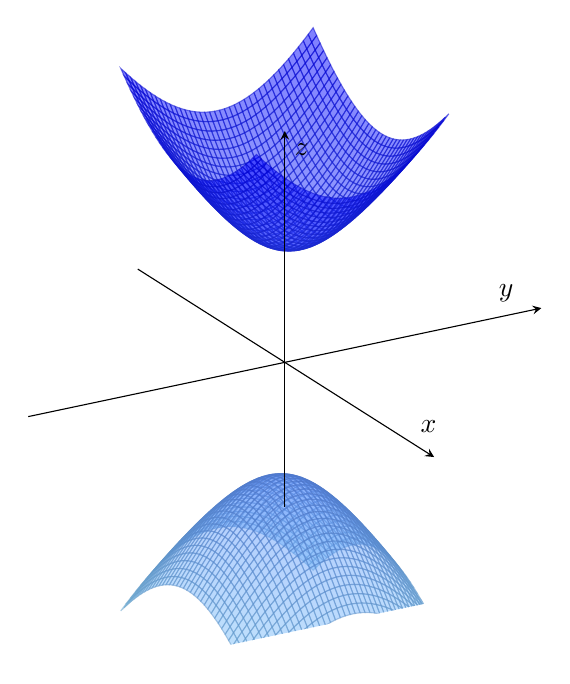
\begin{tikzpicture}
    \begin{axis}[scale=1.5,
        view={60}{30}, % Adjust the viewing angle
        axis lines=center,
        axis on top,
        xlabel={$x$},
        ylabel={$y$},
        zlabel={$z$},
        xmin=-3.25, xmax=3.3,
        ymin=-4, ymax=4,
        zmin=-1.25, zmax=2,
        ticks=none, % Removes the ticks from all axes
        colormap={blues}{color(0cm)=(lightblue); color(1cm)=(blue)} % Define a blue gradient colormap
    ]
    \addplot3[
        surf,
        opacity=0.5, % Adjust the transparency
        samples=40, % Adjust the number of samples for better resolution
        domain=-1.5:1.5, y domain=-1.5:1.5,
        z buffer=sort
    ] ({x},{y},{sqrt(x^2+y^2+1)});
    \addplot3[
        surf,
        opacity=0.5, % Adjust the transparency
        samples=40, % Adjust the number of samples for better resolution
        domain=-1.5:1.5, y domain=-1.5:1.5,
        z buffer=sort
    ] ({x},{y},{-sqrt(x^2+y^2+1)});
    \end{axis}
\end{tikzpicture}
        \label{ch1:fig13}
        \caption{היפרבולואיד דו יריעתי.}
    \end{minipage}
    \hfill % Optional: to ensure horizontal spacing between the plots
    % Second plot
    \begin{minipage}{0.45\textwidth}
        \centering
       \definecolor{lightblue}{rgb}{0.53, 0.81, 0.98}
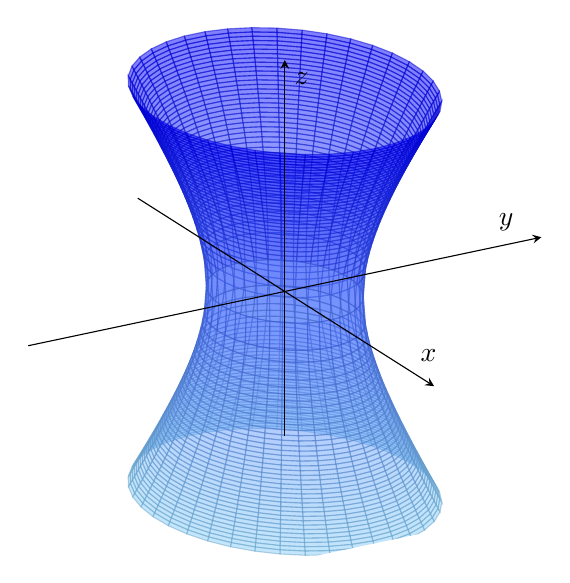
\begin{tikzpicture}
    \begin{axis}[scale=1.5,
        view={60}{30}, % Adjust the viewing angle
        axis lines=center,
        axis on top,
        xlabel={$x$},
        ylabel={$y$},
        zlabel={$z$},
        xmin=-3.25, xmax=3.3,
        ymin=-4, ymax=4,
        zmin=-1.25, zmax=2,
        ticks=none, % Removes the ticks from all axes
        colormap={blues}{color(0cm)=(lightblue); color(1cm)=(blue)} % Define a blue gradient colormap
    ]
    \addplot3[
        surf,
        opacity=0.5, % Adjust the transparency
        samples=40, % Adjust the number of samples for better resolution
        domain=1:2, y domain=0:360,
        z buffer=sort
    ] ({x*cos(y)},{x*sin(y)},{sqrt(x^2-1)});
    \addplot3[
        surf,
        opacity=0.5, % Adjust the transparency
        samples=40, % Adjust the number of samples for better resolution
        domain=1:2, y domain=0:360,
        z buffer=sort
    ] ({x*cos(y)},{x*sin(y)},{-sqrt(x^2-1)});
    \end{axis}
\end{tikzpicture}
		\label{ch1:fig14}
        \caption{היפרבולואיד חד יריעתי.}
    \end{minipage}
\end{figure}

\pagebreak
\section{תרגיל - סיווג קוי רמה}
תארו וציירו את קוי הרמה של הפונקציות הבאות עבור הערכים הנתונים.
\begin{enumerate}
\item קו הרמה של $f(x,y)=\frac{xy}{3x+y-4}$ עבור הערך $C=-1$.
\item מיינו את קווי הרמה של $f(x,y)=\frac{x^2+y^2+2x}{x^2+2y^2+3}$.
\end{enumerate}
\paragraph{פתרון.}
\begin{enumerate}
\item על פי הגדרה, קו הגובה מורכב מאוסף כל הנקודות $\qty(x,y)$ המקיימות $f(x,y)=-1$. כלומר:
\[
	\frac{xy}{3x+y-4}=-1\Longrightarrow xy=4-3x-y\Longrightarrow xy+3x+y-4=0.
\]
כדי לפשט את הביטוי נזהה כי $xy+3x+y+3=(x+1)(y+3)$, ולכן:
\[
	xy+3x+y-4=\qty(x+1)(y+3)-7=0\Longrightarrow (x+1)(y+3)=7.
\]
כלומר, מדובר בהיפרבולה המוזזת כך שראשית הצירים עבורה היא הנקודה $\qty(-1,-3)$, ומסובבת ב-$\frac{\pi}{4}$ רדיאנים נגד כיוון השעון. דרך טובה לצייר אותה היא לחשוב עליה בתוך הגרף של הפונקציה
\[
	y=-3+\frac{7}{x+1}.
\]
\begin{figure}[h]
\begin{center}
 \begin{tikzpicture}
    \begin{axis}[
        axis lines=middle,
        xmin=-7, xmax=5,
        ymin=-12, ymax=9,
        xlabel={$x$},
        ylabel={$y$},
        axis equal, % Ensures equal scaling for x and y axes
        ticks=none, % Removes the ticks from both axes
        samples=200
    ]

    % Draw the hyperbola
    \addplot[blue, thick, domain={-1+7/9}:8] ({x},{-3+7/(x+1)});
	\addplot[blue, thick, domain=-10:{-1-7/9}] ({x},{-3+7/(x+1)});
	
    % Draw rotated axis lines
    \addplot[blue, dashed, domain=-10:8] ({x},{x-2});
	\addplot[blue, dashed, domain=-10:8] ({x},{-x-4});	
	
	% Origin for the Hyperbola
    \coordinate (P) at (-1,-3);
    \fill[purple] (P) circle (2pt) node[below right, black]{$(-1,-3)$};
    	
    \end{axis}
\end{tikzpicture}
\label{ch1:fig16}
\caption{איור של ההיפרבולה $(x+1)(y+3)=7$, ראשית הצירים המוזזת ב-$(-1,-3)$ והישרים $y=x-2,-x-4$.}
\end{center}
\end{figure}
\item על פי הגדרה, עלינו לפתור את המשוואה
\[
	\frac{x^2+y^2+2x}{x^2+2y^2+3}=C
\]
עבור כל הערכים האפשריים של $C$. לאחר סידור המשוואה מקבלים
\[
	\qty(1-C)x^2+2x+\qty(1-2C)y^2=3C,
\]
תחילה, נפתור עבור המקרה שבו $C=1$, ובמקרה זה נקבל את המשוואה $-y^2=3$, וקו הרמה המתאים יהיה \textbf{קבוצה ריקה}. אחרת, ניתן לבצע השלמה לריבוע באופן הבא:
\[
	\qty(1-C)\qty(x+\frac{1}{1-C})^2+\qty(1-2C)y^2=\frac{3C-3C^2+1}{1-C}.
\]
עתה, הצורה שתתקבל תקבע על פי הסימנים השונים של המקדמים ולכן נזהה את ערכי $C$ שבהם סימני המקדמים מתחלפים, ואלו הם
\[
	C=1,C=\frac{1}{2},C=\frac{1}{2}+\sqrt{\frac{7}{12}}\approx 1.26,C=\frac{1}{2}-\sqrt{\frac{7}{12}}\approx -0.26.
\]
\begin{enumerate}
\item כאשר $C>\frac{1}{2}+\sqrt{\frac{7}{12}}$, המקדמים באגף השמאלי שליליים והמקדם באגף הימני חיובי. במקרה זה, קו הרמה תהיה \textbf{קבוצה ריקה}.
\item כאשר $C=\frac{1}{2}+\sqrt{\frac{7}{12}}$, המקדמים באגף השמאלי שווי סימן (שליליים) ובאגף הימני מקבלים אפס. במקרה זה, קו הרמה יהיה \textbf{נקודה בודדת}, והיא הנקודה $\qty(-\frac{1}{\frac{1}{2}-\sqrt{\frac{7}{12}}},0)$.
\item כאשר $1<C<\frac{1}{2}+\sqrt{\frac{7}{12}}$, כל מקדמי המשוואה בעלי סימן זהה אך המקדמים באגף השמאלי שונים אחד מהשני. הצורה שתתקבל היא \textbf{אליפסה}.
\item כאשר $\frac{1}{2}<C<1$ מקבלים כי המקדם של $\qty(x+\frac{1}{1-C})^2$ חיובי אך יתר המקדמים שליליים, ולכן מדובר ב\textbf{היפרבולה שוכבת}.
\item כאשר $C=\frac{1}{2}$ מקבלים את המשוואה
\[
	\frac{1}{2}\qty(x+2)^2=\frac{7}{2}\Longrightarrow x=-2\pm\sqrt{7}.
\]
לכן, קו הרמה יהיה \textbf{שני ישרים מקבילים}.
\item כאשר $\frac{1}{2}-\sqrt{\frac{7}{12}}<C<\frac{1}{2}$ כל המקדמים של המשוואה חיוביים ולכן מתקבלת \textbf{אליפסה} למעט במקרה שבו $C=0$ ואז מתקבל \textbf{מעגל}.
\item כאשר $C=\frac{1}{2}-\sqrt{\frac{7}{12}}$ מקבלים כי המקדמים באגף השמאלי חיוביים והמקדם באגף הימני מתאפס, ולכן קו הרמה יהיה \textbf{נקודה בודדת}, והיא הנקודה $\qty(-\frac{1}{\sqrt{\frac{7}{12}}-\frac{1}{2}},0)$.
\item כאשר $C<\frac{1}{2}-\sqrt{\frac{7}{12}}$ המקדמים באגף השמאלי חיוביים בעוד המקדם באגף הימני שלילי, ולכן קו הרמה יהיה \textbf{קבוצה ריקה}.
\end{enumerate}
\begin{figure}[h]
\begin{center}
 \begin{tikzpicture}
    \begin{axis}[
        axis lines=middle,
        xmin=-18, xmax=9,
        ymin=-9, ymax=10,
        xlabel={$x$},
        ylabel={$y$},
        axis equal, % Ensures equal scaling for x and y axes
        ticks=none, % Removes the ticks from both axes
        samples=200
    ]

    % C=1.2
    \addplot[blue, thick, domain=0:2*pi] ({5+sqrt(7)*cos(deg(x))},{sin(deg(x))}) node[below, black] {$\mbox{(ג)}$};
    
    % C=0.8
    \addplot[blue, thick, domain=-7:7] ({-5+sqrt(37+3*(x^2))},{x}) node[above left, black]{$\mbox{(ד)}$};
    \addplot[blue, thick, domain=-7:7] ({-5-sqrt(37+3*(x^2))},{x}) node[above right, black]{$\mbox{(ד)}$};
	
	% C=0.5
    \addplot[blue, thick, domain=0:9] ({-2+sqrt(7)},{x}) node[midway, right, black]{$\mbox{(ה)}$};
    \addplot[blue, thick, domain=0:9] ({-2-sqrt(7)},{x}) node[midway, left, black]{$\mbox{(ה)}$};
    \addplot[blue, thick, domain=-9:0] ({-2+sqrt(7)},{x});
    \addplot[blue, thick, domain=-9:0] ({-2-sqrt(7)},{x});
    
    % C=0.2
    \addplot[blue, thick, domain={pi/2}:{5*pi/2}] ({-(4/3)+(5/3)*cos(deg(x))},{(5/sqrt(6))*sin(deg(x))}) node[above,black]{$\mbox{(ו)}$};
	
	% C=0.5+sqrt(7/12)
    \coordinate (P1) at ({-1/(0.5-sqrt(7/12))},0);
    \fill[blue] (P1) circle (2pt) node[below, black]{$\mbox{(ב)}$};
    
    % C=0.5-sqrt(7/12)
    \coordinate (P2) at ({-1/(0.5+sqrt(7/12))},0);
    \fill[blue] (P2) circle (2pt) node[below, black]{$\mbox{(ז)}$};
    	
    \end{axis}
\end{tikzpicture}
\label{ch1:fig17}
\caption{תיאור קוי הרמה (שאינם קבוצות ריקות) של הפונקציה $f(x,y)=\frac{x^2+y^2+2x}{x^2+2y^2+3}$.}
\end{center}
\end{figure}
\end{enumerate}
\section{תרגיל - הצגות פרמטריות}
\begin{enumerate}
\item נסמן ב-$S$ את החרוט $x^2+y^2-z^2=0$. הראו כי לכל נקודה $\qty(x_0,y_0,z_0)\in S$ ניתן למצוא ישר העובר בנקודה זו ומוכל כולו ב-$S$.
\item מצאו שני משטחים ריבועיים המכילים את כל הנקודות מהצורה 
\[
(\cos^2{(\theta)},\sin{(\theta)}\cos{(\theta)},\sin{(\theta)})
\]
 כאשר $\theta\in\qty[0,2\pi]$.
\end{enumerate}
\paragraph{פתרון.}
\begin{enumerate}
\item כדי להתחיל להתמודד עם השאלה, נזכיר כי ישר ב-$\bR^3$ מאופיין באופן יחיד על פי נקודה שהוא עובר דרכה והכיוון שלו שמתואר על ידי וקטור כלשהו $(a,b,c)$. כלומר, ניתן להציג כל ישר העובר דרך הנקודה הנתונה בצורה הפרמטרית
\begin{multline*}
	\qty(x(t),y(t),z(t))=\qty(x_0+at,y_0+bt,z_0+ct)=\qty(x_0,y_0,z_0)+t(a,b,c),\\ t\in\bR.
\end{multline*}
דרגות החופש של הבעיה יהיו הפרמטרים $(a,b,c)$ שיקבעו על פי התנאי הנוסף שדרשו מאיתנו בשאלה - לוודא כי הישר מוכל כולו במשטח. כדי לעשות זאת אין לנו הרבה ברירה, אלא להציב את נקודות הישר במשוואה שמגדירה את המשטח $S$ ולוודא שהמשוואה מתקיימת לכל $t$, כלומר
\[
	\qty(x_0+at)^2+\qty(y_0+bt)^2-\qty(z_0+ct)^2=0.
\]
לאחר פתיחת סוגריים וסידור מחדש של המשוואה, מקבלים כי הישר יהיה מוכל במשטח אם ורק אם
\begin{multline*}
	\qty(x_0^2+y_0^2-z_0^2)+2\qty(ax_0+by_0-cz_0)t+\qty(a^2+b^2-c^2)t^2=0, \\ \forall t\in\bR.
\end{multline*}
שימו לב כי הביטוי שקיבלנו הוא פולינום ממעלה $2$ (ב-$t$) שמתאפס לכל ערך של $t$, ולכן חייב להיות פולינום האפס, כלומר כל מקדמי הפולינום מתאפסים, ומכאן מערכת המשוואות:
\[
	\left\{\begin{array}{l}
	x_0^2+y_0^2-z_0^2=0 \\
	ax_0+by_0-cz_0=0 \\
	a^2+b^2-c^2=0
	\end{array}\right..
\]
עתה, נוכל להשתמש בנתון כי $\qty(x_0,y_0,z_0)\in S$ כדי להסיק שהמשוואה הראשונה מתקיימת בכל מקרה, ועלינו למצוא $(a,b,c)$ המקיימים את זוג המשוואות האחרונות. במקרה זה, ניתן לפתור את המשוואות בצורה ריגורוזית על ידי בידוד משתנים והצבה, אך למעשה התבוננות קצרה תראה שהבחירה
\[
	\qty(a,b,c)=\qty(x_0,y_0,z_0)
\]
מקיימת את הדרוש\footnote{יחד עם זאת, בהחלט מומלץ לנסות ולפתור את המשוואות בצורה יסודית לשם תרגול נוסף ולראות שאכן מתקבלת אותה התשובה.}. יתרה מכך, כל כפולה בסקלר של וקטור פרמטרים זה תהווה תשובה נכונה (חשבו מדוע!).
\item כפי שראינו, משטחים ריבועיים רבים מערבים את $x^2,y^2,z^2$ בקומבינציות שונות. לכן, דרך טובה לחפש את המשטחים המבוקשים תהיה לחשב את שלושת הביטויים הללו ולנסות למצוא קומבינציות שלהם שיתנו את הערך אפס לכל $\theta$. במקרה שלנו:
\[
	x^2\qty(\theta)=\cos^4{(\theta)},\quad y^2\qty(\theta)=\sin^2{(\theta)}\cos^2{(\theta)},\quad z^2\qty(\theta)=\sin^2{(\theta)}
\]
עתה, שימוש פשוט בזהויות טריגונומטריות יראה לנו כי:
\[
	x^2\qty(\theta)+y^2\qty(\theta)=\cos^2{\qty(\theta)}\qty(\cos^2{(\theta)}+\sin^2{(\theta)})=\cos^2{(\theta)}=x\qty(\theta).
\]
כלומר, כל הנקודות הנתונות נמצאות על הגליל $x^2+y^2=x$, והוספה של $z^2\qty(\theta)$ למשוואה תראה כי כל הנקודות נמצאות גם על ספירת היחידה $x^2+y^2+z^2=1$. כמובן שלא מדובר בשני המשטחים היחידה שמכילים את הנקודות, ומומלץ לנסות למצוא משטחים נוספים כתרגיל. באיור \ref{ch1:fig18} ניתן לראות את שני המשטחים ואת \linebreak אוסף הנקודות (המהוות בדיוק את החיתוך בין שני המשטחים). חיתוך זה הינו עקום מפורסם הידוע בשם "החלון של ויויאני"\footnote{וינצ'נזו ויויאני היה מתמטיקאי ומדען איטלקי, ותלמידו של גלילאו. ויויאני היה הראשון שניסה לערוך ולפרסם את אוסף עבודותיו של גלילאו, ומאמציו נעצרו עקב התנגדות הכנסיה הקתולית.}. לעקום זה מספר תכונות גיאומטריות מעניינות, וביניהן העובדה שהצל שהוא מטיל בכיוון ציר ה-$x$ יוצר צורת $8$ הידועה בשם "הלמניסקטה".
\begin{figure}[h]
\begin{center}
\definecolor{lightblue}{rgb}{0.53, 0.81, 0.98}
\definecolor{lightred}{rgb}{1, 0.7, 0.7}
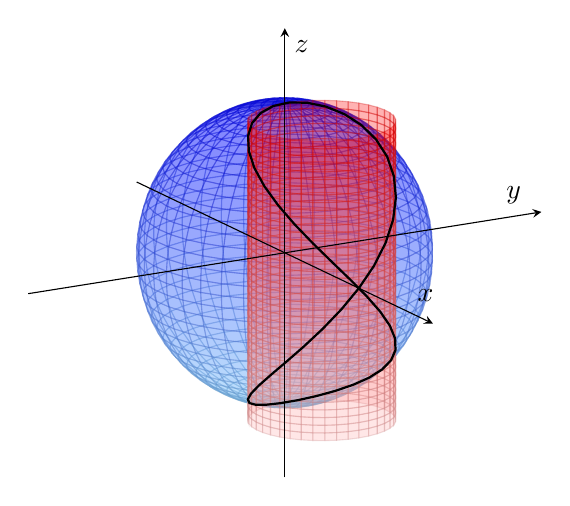
\begin{tikzpicture}
    \begin{axis}[scale=1.5,
        view={60}{20}, % Adjust the viewing angle
        axis lines=center,
        axis on top,
        xlabel={$x$},
        ylabel={$y$},
        zlabel={$z$},
        xmin=-2, xmax=2,
        ymin=-2, ymax=2,
        zmin=-1.5, zmax=1.5,
        ticks=none, % Removes the ticks from all axes
    ]
    % Define the colormaps
    \pgfplotsset{
        colormap={blues}{color(0cm)=(lightblue); color(1cm)=(blue)}, % Blue gradient colormap
        colormap={reds}{color(0cm)=(lightred); color(1cm)=(red)} % Red gradient colormap
    }

    % Unit sphere with blue gradient
    \addplot3[
        surf,
        colormap name=blues, % Use the blue gradient colormap
        opacity=0.3,
        samples=40,
        domain=0:2*pi, y domain={-pi/2}:{pi/2},
        z buffer=sort
    ] ({cos(deg(y))*cos(deg(x))},{cos(deg(y))*sin(deg(x))},{sin(deg(y))});

    % Cylinder with red gradient
    \addplot3[
        surf,
        colormap name=reds, % Use the red gradient colormap
        opacity=0.3,
        samples=40,
        domain=0:2*pi, y domain=-1:1,
        z buffer=sort
    ] ({0.5+0.5*cos(deg(x))},{0.5*sin(deg(x))},{y});

    % Curve with the given parametrization
    \addplot3[
        thick,
        samples=50,
        domain=0:2*pi
    ] ({cos(deg(x))^2},{sin(deg(x))*cos(deg(x))},{sin(deg(x))});

\end{axis}
\end{tikzpicture}
\label{ch1:fig18}
\caption{תיאור ספירת היחידה, הגליל ואוסף הנקודות הנתון בשאלה.}
\end{center}
\end{figure}
\end{enumerate}
\section{תרגיל - סיווג משטחי רמה}

